\documentclass[12pt,fleqn]{report} %taille de la police par défaut, et équations jusitifées à gauche
\usepackage[left=2cm,right=2cm,top=2cm,bottom=2cm,headsep=10pt,a4paper]{geometry}
\usepackage{xcolor}
\definecolor{enstabGreen}{HTML}{C8D200} 	%vert  	#c8d200 
\definecolor{enstabLightGreen}{HTML}{E9ED99} 	%vert  	#c8d200 
\definecolor{enstabLightBlue}{HTML}{009EE0} %bleu clair 	#009ee0
\definecolor{enstabVeryLightBlue}{HTML}{99D8F3} %bleu clair 	#009ee0
\definecolor{enstabDarkBlue}{HTML}{005C8F}	%bleu foncé 	#005c8f
\definecolor{enstabDarkGrey}{HTML}{333333}	%gris fort 	#333333
\definecolor{enstabLightGrey}{RGB}{48,48,48}	%gris fort 	#333333
\definecolor{enstabParme}{HTML}{8878B2}		%parme 	#8878b2
\definecolor{enstabOrange}{HTML}{F18E00} 	%orange 	#f18e00
\usepackage[colorlinks=true,
        urlcolor=enstabLightBlue,
        anchorcolor=enstabDarkBlue,
        linkcolor=enstabDarkBlue,
        citecolor=enstabDarkGrey,
        pdfauthor={O. Reynet},
        pdfkeywords={LaTeX; Report},
        pdftitle={How to produce a report with LaTeX},
        pdfsubject={yours !}] {hyperref}
\usepackage{url}
\usepackage[utf8]{inputenc} % lettres accentuées
\usepackage[T1]{fontenc}    % Use 8-bit encoding that has 256 glyphs
\usepackage[UKenglish]{babel} % Pour le français
\usepackage{eso-pic}        % pour une image en fond, page de titre
\usepackage{graphicx}       % Pour inclure des images
\graphicspath{{images/}}    % Où sont les images ?

\usepackage{listings}      % Pour coloriser les codes que vous insérez
\lstset{ %
  backgroundcolor=\color{white},   % choose the background color; you must add \usepackage{color} or 
  basicstyle=\footnotesize\ttfamily,        % the size of the fonts that are used for the code
  breakatwhitespace=false,         % sets if automatic breaks should only happen at whitespace
  breaklines=true,                 % sets automatic line breaking
  captionpos=b,                    % sets the caption-position to bottom
  commentstyle=\color{enstabOrange},    % comment style
  deletekeywords={...},            % if you want to delete keywords from the given language
  escapeinside={\%*}{*)},          % if you want to add LaTeX within your code
  extendedchars=true,              % lets you use non-ASCII characters; for 8-bits encodings only, does not work with UTF-8
  %frame=single,                    % adds a frame around the code
  keepspaces=true,                 % keeps spaces in text, useful for keeping indentation of code (possibly needs columns=flexible)
  keywordstyle=\color{enstabDarkBlue},       % keyword style
  %language=Octave,                 % the language of the code
  morekeywords={*,...},            % if you want to add more keywords to the set
  numbers=left,                    % where to put the line-numbers; possible values are (none, left, right)
  numbersep=8pt,                   % how far the line-numbers are from the code
  numberstyle=\tiny\color{enstabDarkGrey}, % the style that is used for the line-numbers
  rulecolor=\color{black},         % if not set, the frame-color may be changed on line-breaks within not-black text (e.g. comments (green here))
  showspaces=false,                % show spaces everywhere adding particular underscores; it overrides 'showstringspaces'
  showstringspaces=false,          % underline spaces within strings only
  showtabs=false,                  % show tabs within strings adding particular underscores
  stepnumber=5,                    % the step between two line-numbers. If it's 1, each line will be numbered
  stringstyle=\color{enstabParme},     % string literal style
  tabsize=2,                       % sets default tabsize to 2 spaces
  title=\lstname                   % show the filename of files included with \lstinputlisting; also try caption instead of title
}





\usepackage{booktabs}       % pour de jolis tableaux
%\usepackage{fancyhdr}       % pour des entêtes et pieds de pages améliorés.
\usepackage{makeidx}        % requis pour faire les index
\usepackage{amsmath}
\usepackage{amsfonts}
\usepackage{amssymb}
\usepackage{color}
\usepackage{array}
\usepackage{graphicx}
\usepackage{caption} 
\usepackage{hyperref}
\usepackage{algorithm}
\usepackage{algorithmic}
\usepackage{times}
\usepackage{tabularx}     % Ce fichier contient tous les packages nécessaires à la compilation
\makeindex           % donne l'ordre de créer l'index

\begin{document}
\renewcommand{\contentsname}{Contents}                % des jolis noms pour la table des matières
\renewcommand{\bibname}{Bibliography}  % des jolis noms pour les sections bibliographiques

%----------------------------------------------------------------------------------------
%	 PAGE DE TITRE
%-----------------------------	-----------------------------------------------------------

\begingroup
\thispagestyle{empty}
\AddToShipoutPicture*{\put(6,5){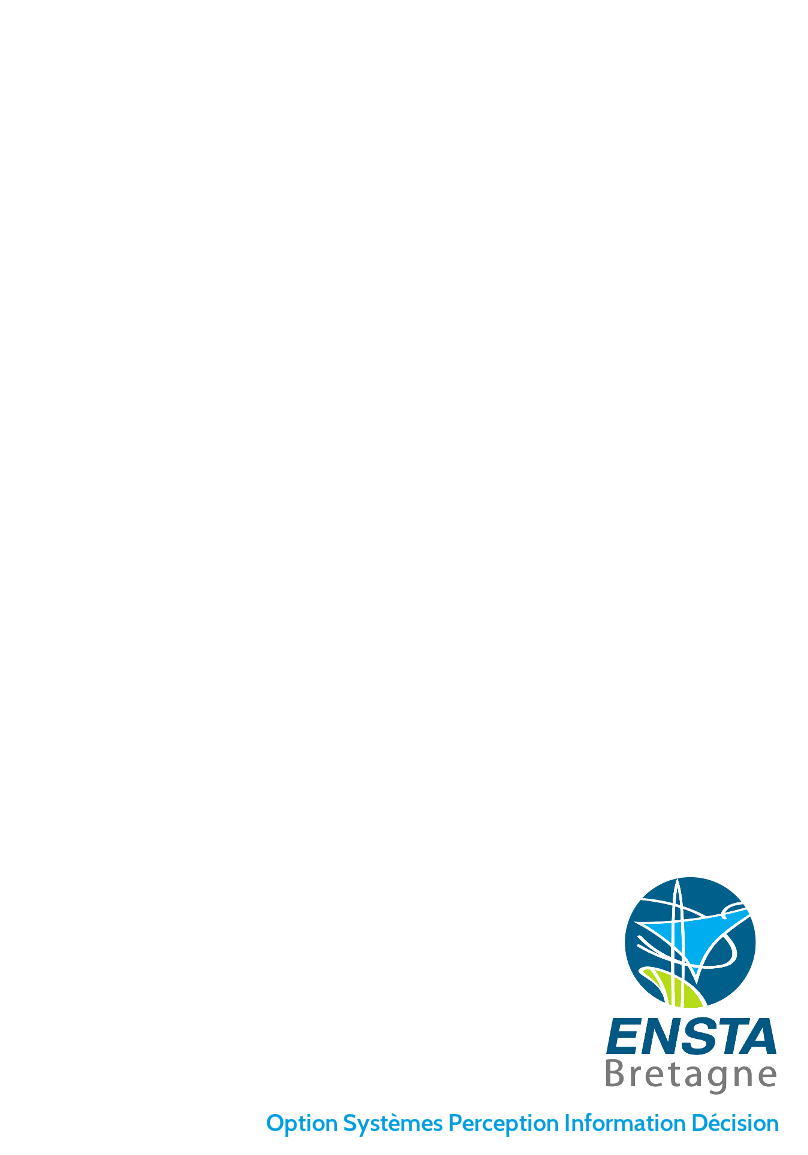
\includegraphics[scale=1]{Images/FondTitreSPID}}} % Image background
\begin{center}
\vspace*{2cm}
{\Huge \textsc{\textbf{Status Report}}}\\


\vspace*{2cm}
{\huge Realization of an autonomous sail-boat}\par % Intitulé du projet
\end{center}
%\begin{figure}[H]
%\centering
%    \includegraphics[trim={1cm 1cm 0.7cm 5cm},clip, scale=0.6]{biscay.png}
%\end{figure}

\vspace*{1.5cm}
\textbf{\large Written by:} 
\begin{center}
{\large
\begin{tabular}{cc}
\\
\\
\\
Philippe Chuzel\\
\\
\\
\end{tabular}}
\end{center}


%\vspace*{1.5 cm}
%{\large \textbf{Under the supervision of:}}\\
%\begin{center}
%{\large
%Jean-Christophe Cexus\\
%Arnaud Coatanhay\\}
%\end{center}
\endgroup


%----------------------------------------------------------------------------------------
%	SOMMAIRE
%----------------------------------------------------------------------------------------
\tableofcontents  % Imprime le sommaire
\cleardoublepage  % pour commencer sur une page impaire

\chapter*{Abstract}
\input{Abstract}

\chapter*{Introduction}
The purpose of this project is to analyse the electromagnetic signature of object when its form changes during time. The electromagnetic signature analysis is a common subject for people who work in the filed of radar detection. However, the study of object signature which its form change through time is still full of many questions which have not been answered. The study of those object imply to do a very strict analyse of the electronic signature thanks to the time frequency analysis tools.

\bigskip

During this project \cite{Analysis}, we have to look at the different tools which can help us to analyse the electronic signature of an object and to help us to understand the effects of change of shape of an object. The final deliverable expected is a set of program which can allow us to implement an entire loop of treatment. This loop has to help us to understand how an object deformed according to the modification of its electronic signature. \textbf{All the code had to be done in python} which imply that some function had to be implemented by ourself. A lot of documentation have been given by the supervisor  but only have

\bigskip

The whole project code and result can be find here :

\textit{https://github.com/chuzelph-ENSTA-Bretagne/TFR \_ Deform.git}


\begin{figure}[H]
\centering
    \includegraphics[scale=1,angle=0]{Images/Image1.PNG}
    \caption{General situation of our subject.}
    \label{fig:Image1}
\end{figure}

\bigskip

The first part will try to explain which equations have to be understood in order to get the analytic expression of the electromagnetic field coming from the object.
The second part will expose the different tools which have been create for the time frequency analysis that can be used for this project. During this part, some simple signals will be used in order to represent the results that can be obtain with those tools.
The last part will present the tools which have been develop in order to extract information from the time/frequency representation in order to find correlation between the deformation of the object and the variation of the electromagnetic field.



%----------------------------------------------------------------------------------------
%	PART I 
%----------------------------------------------------------------------------------------
\part{Regulation}
\chapter{Sailboat regulation}


The original algorithms which were used in order to regulate a sail-boat is given here
\cite{jaulin2015robotique}.

For all those algorithms, we decide to chose one specific situation and we express the regulator in order to generate a potential adapted to the situation. For example, the following algorithm is used for the line regulation of the sail-boat \ref{alg:MYALG_line}.

\begin{algorithm}[H]
  \caption{Sail-boat regulator , line }
  \label{alg:MYALG_line}
  \textbf{Inputs}% Inputs section
  \begin{algorithmic}[1]
    \STATE $m$ position of the sailboat
    \STATE $\theta$ heading of the sail-boat
    \STATE $\psi$ wind direction
    \STATE $a,b$ point of the line
    \STATE $q$ hysteresis
  \end{algorithmic}
  \bigskip

  \textbf{Output}% Output section
  \begin{algorithmic}[1]
    \STATE $\delta_r$ ruder angle
    \STATE $\delta_s$ sail angle
    \STATE $q$ hysteresis
  \end{algorithmic}
  \bigskip
  
  \textbf{Initialization}% Initialization section
  \begin{algorithmic}[1]
   	\STATE $q\gets 1$
  \end{algorithmic}
  
  
  \textbf{Algorithm}
  \begin{algorithmic}[1]
  	\STATE $e = det(\frac{b-a}{||b-a||},m-a)$
  	
  		\IF{$|e|>\frac{r}{2}$}
  			\STATE q = sign(e)
  		\ENDIF
  		
  		\STATE $\varphi = atan2(b-a)$
  		\STATE $\theta^* = \varphi - \frac{2\gamma_{\infty}}{\pi} . atan(\frac{e}{r})$
	 	\IF{ cos($\psi$-$\theta^*$)+cos($\zeta$) < 0 or ($|e|<r$ and cos($\psi$-$\varphi$)  + cos($\zeta$))}
     	  	\STATE $\theta_p$ = $\pi$ + $\psi$ - q . $\zeta$
     	
		\ELSE
			\STATE $\theta_p$ = $\theta^*$
	 	\ENDIF
	 	
  \STATE $\delta_r$ = $\frac{\delta_s^{max}}{\pi} . atan(tan(\frac{\theta-\theta_p}{2}))$
  
  \STATE $\delta_s$ = $\delta_s^{max} . \frac{cos(\psi-\theta_p)+1}{2}$
	
  \end{algorithmic}
\end{algorithm}

In the end, we generate a field potential as below which allow the sail-boat to follow the line.

\begin{figure}[H]
\centering
    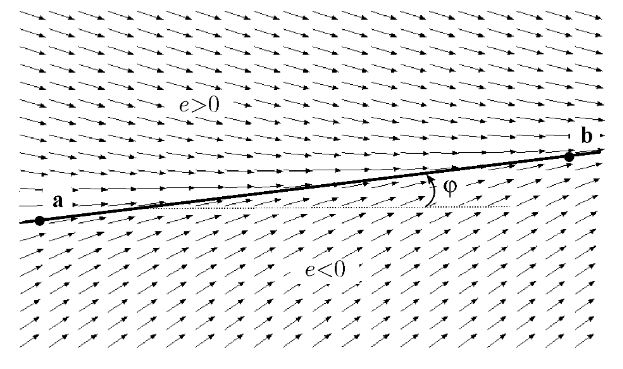
\includegraphics[scale=0.5,angle=0]{Images/FieldVector.png}
    \caption{Field potential generated by this regulator.}
    \label{fig:FieldVector}
\end{figure}


\chapter{Generation of field potential}


Nevertheless, we wanted to realize a new version of this algorithm which would allow us to get the value of the ruder angle and the sail angle by only providing the heading wanted, the real heading and the wind direction. 




\chapter{update of the algorithm}

The following algorithm is the result of our work \ref{alg:MYALG}.


\begin{algorithm}[H]
  \caption{Sail-boat regulator V1 }
  \label{alg:MYALG}
  \textbf{Inputs}% Inputs section
  \begin{algorithmic}[1]
    \STATE $\theta^*$ heading wanted
    \STATE $\theta$ heading of the sail-boat
    \STATE $\psi$ wind direction
    \STATE q hysteresis
  \end{algorithmic}
  \bigskip

  \textbf{Output}% Output section
  \begin{algorithmic}[1]
    \STATE $\delta_r$ ruder angle
    \STATE $\delta_s$ sail angle
    \STATE q hysteresis
  \end{algorithmic}
  \bigskip
  
  \textbf{Initialization}% Initialization section
  \begin{algorithmic}[1]
   	\STATE $q\gets 1$
  \end{algorithmic}
  
  
  \textbf{Algorithm}
  \begin{algorithmic}[1]
	 	\IF{ cos($\psi$-$\theta^*$)+cos($\zeta$) < 0}
	 		\STATE q = sign(sin($\psi-\theta^*$))
     	  	\STATE $\theta_p$ = $\pi$ + $\psi$ - q . $\zeta$
     	
		\ELSE
			\STATE $\theta_p$ = $\theta^*$
	 	\ENDIF
	 	
  \STATE $\delta_r$ = $\frac{\delta_s^{max}}{\pi} . atan(tan(\frac{\theta-\theta_p}{2}))$
  
  \STATE $\delta_s$ = $\delta_s^{max} . \frac{cos(\psi-\theta_p)+1}{2}$
	
  \end{algorithmic}
\end{algorithm}






%----------------------------------------------------------------------------------------
%	PART II 
%----------------------------------------------------------------------------------------
\part{A voir}


\chapter{Presentation of the sail-boat}

put photos here!!!

\chapter{Choice of the component}


\section{Rasberry Pi}

\begin{figure}[H]
\centering
    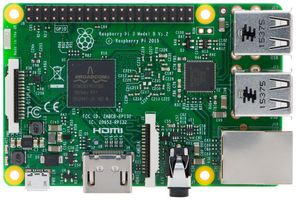
\includegraphics[scale=0.5,angle=0]{Images/RasberryPy2.jpg}
    \caption{Rasberry Pi nuke.}
    \label{fig:Rasberry}
\end{figure}


\section{IMU Razor}

\begin{figure}[H]
\centering
    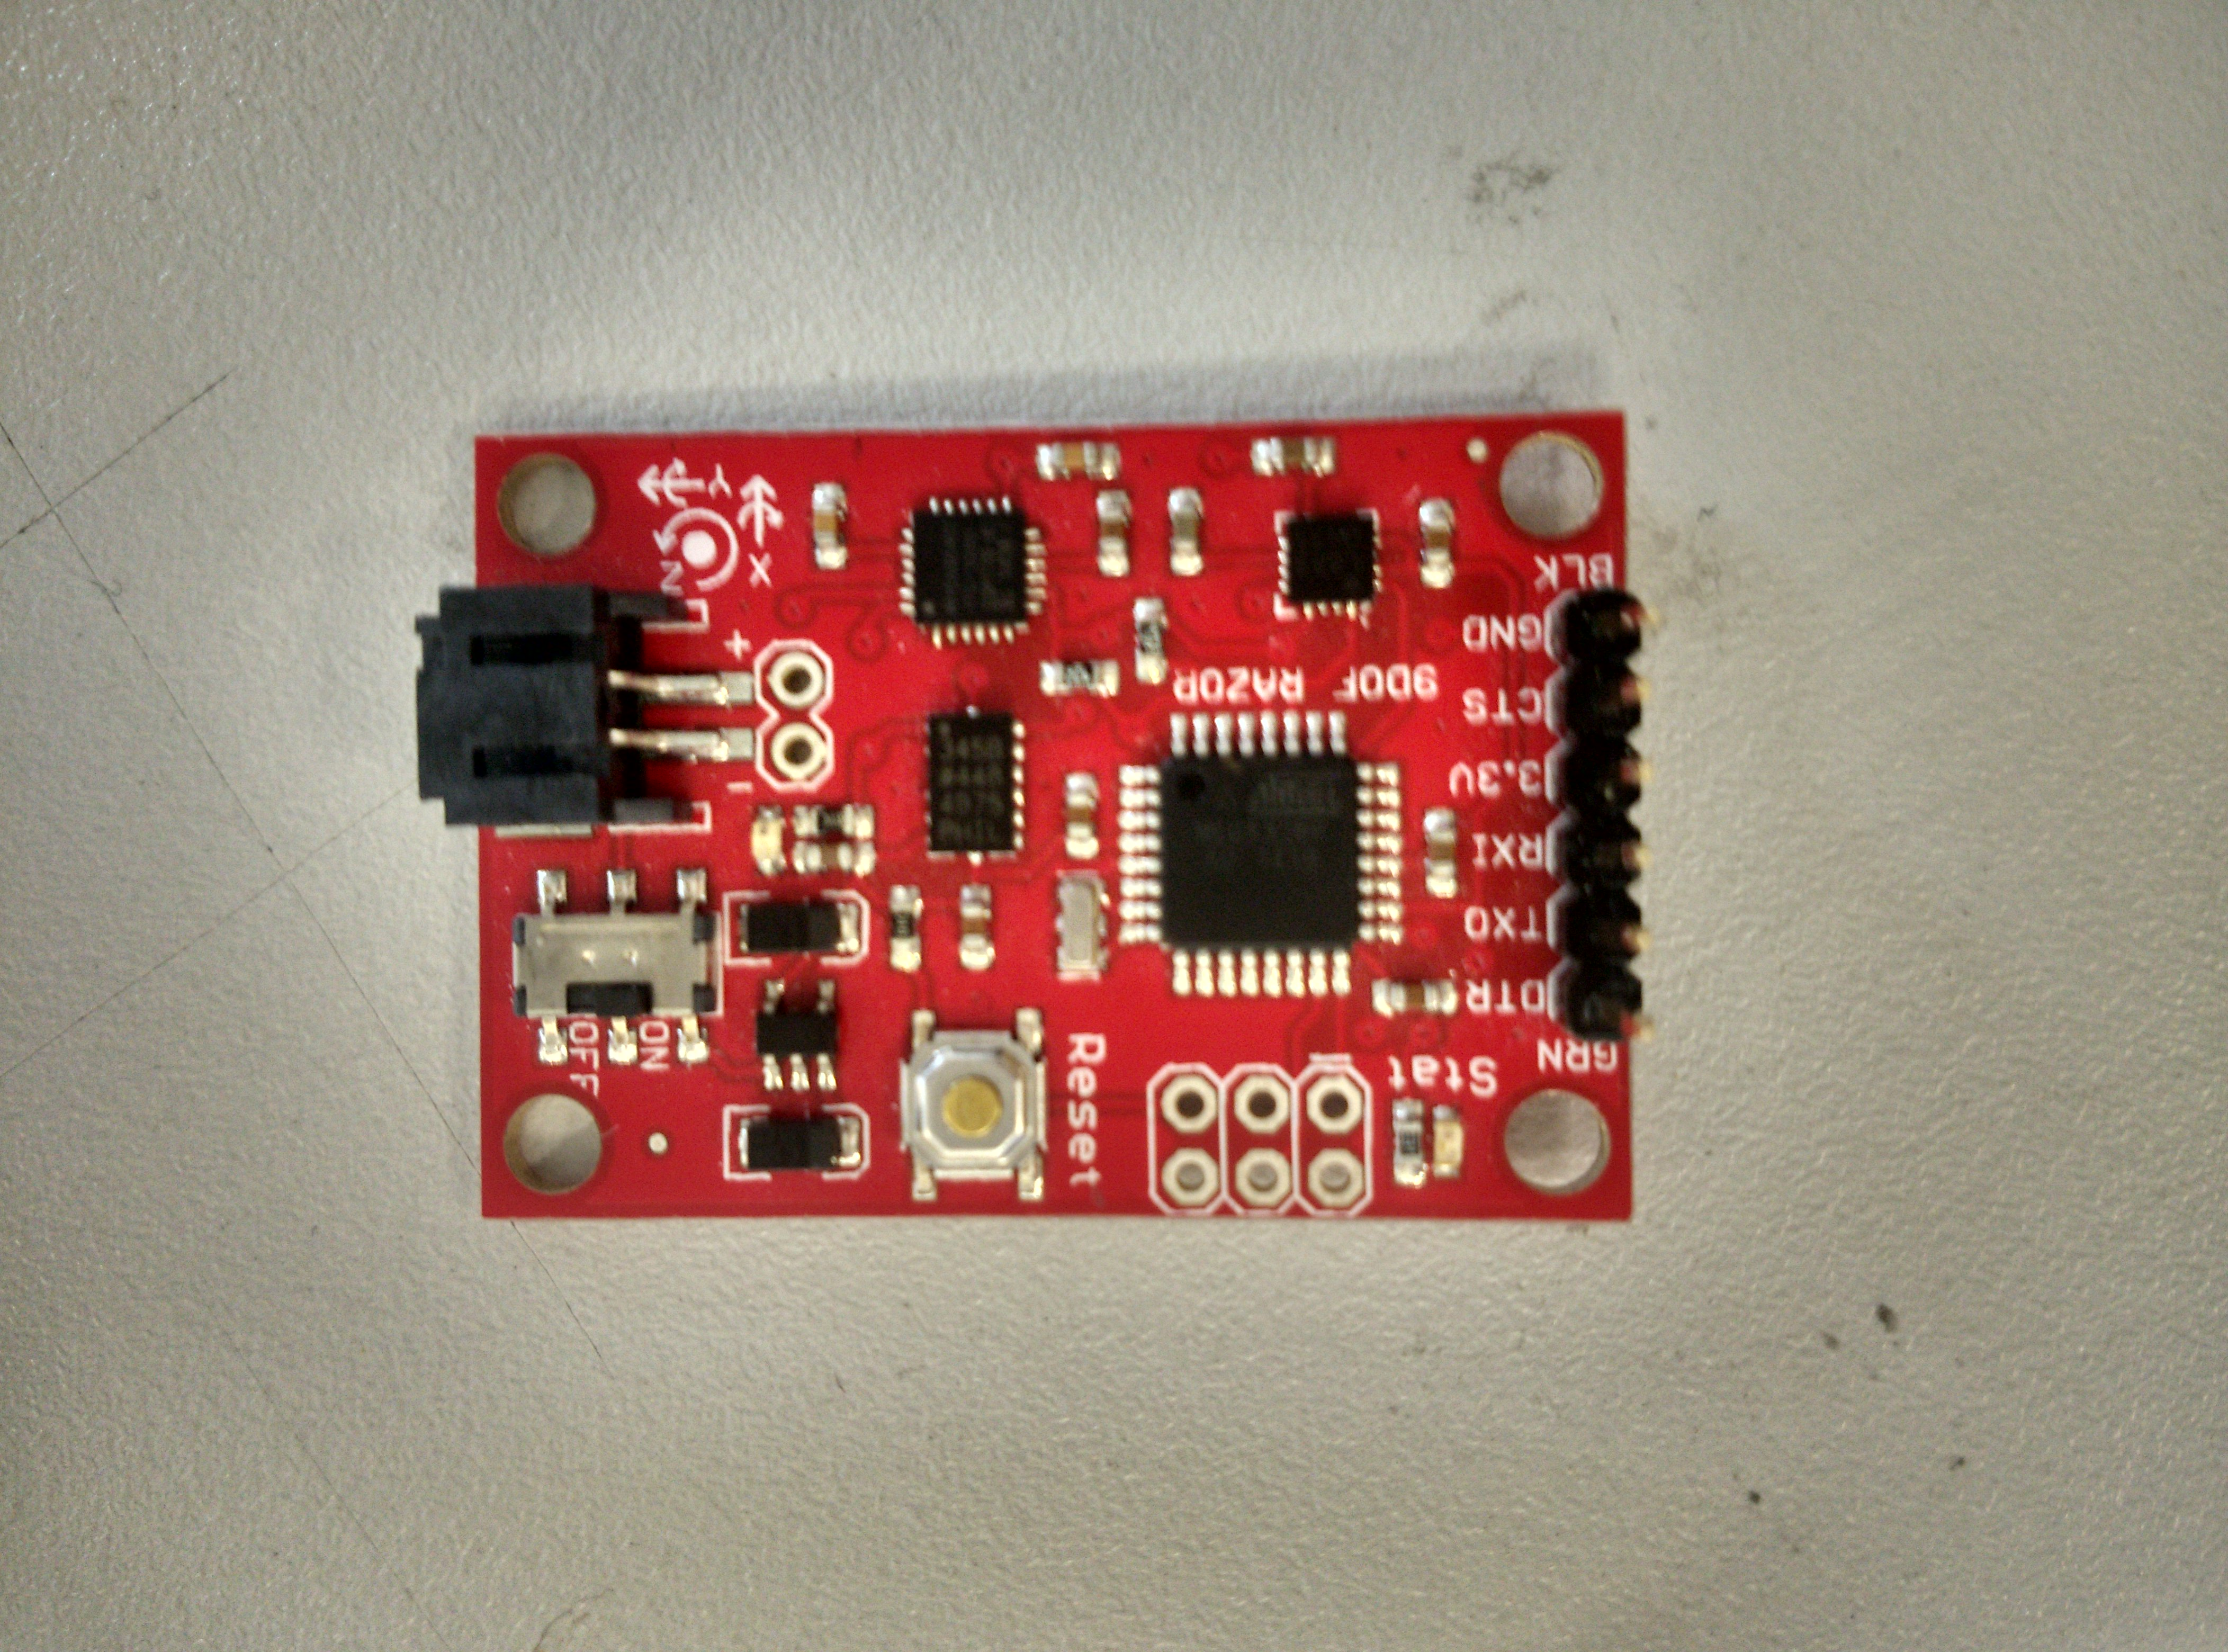
\includegraphics[scale=0.05,angle=0]{Images/RazorIMU.jpg}
    \caption{Razor IMU.}
    \label{fig:RazorIMU}
\end{figure}


\section{Magnetic stator, wind captor}

\begin{figure}[H]
\centering
    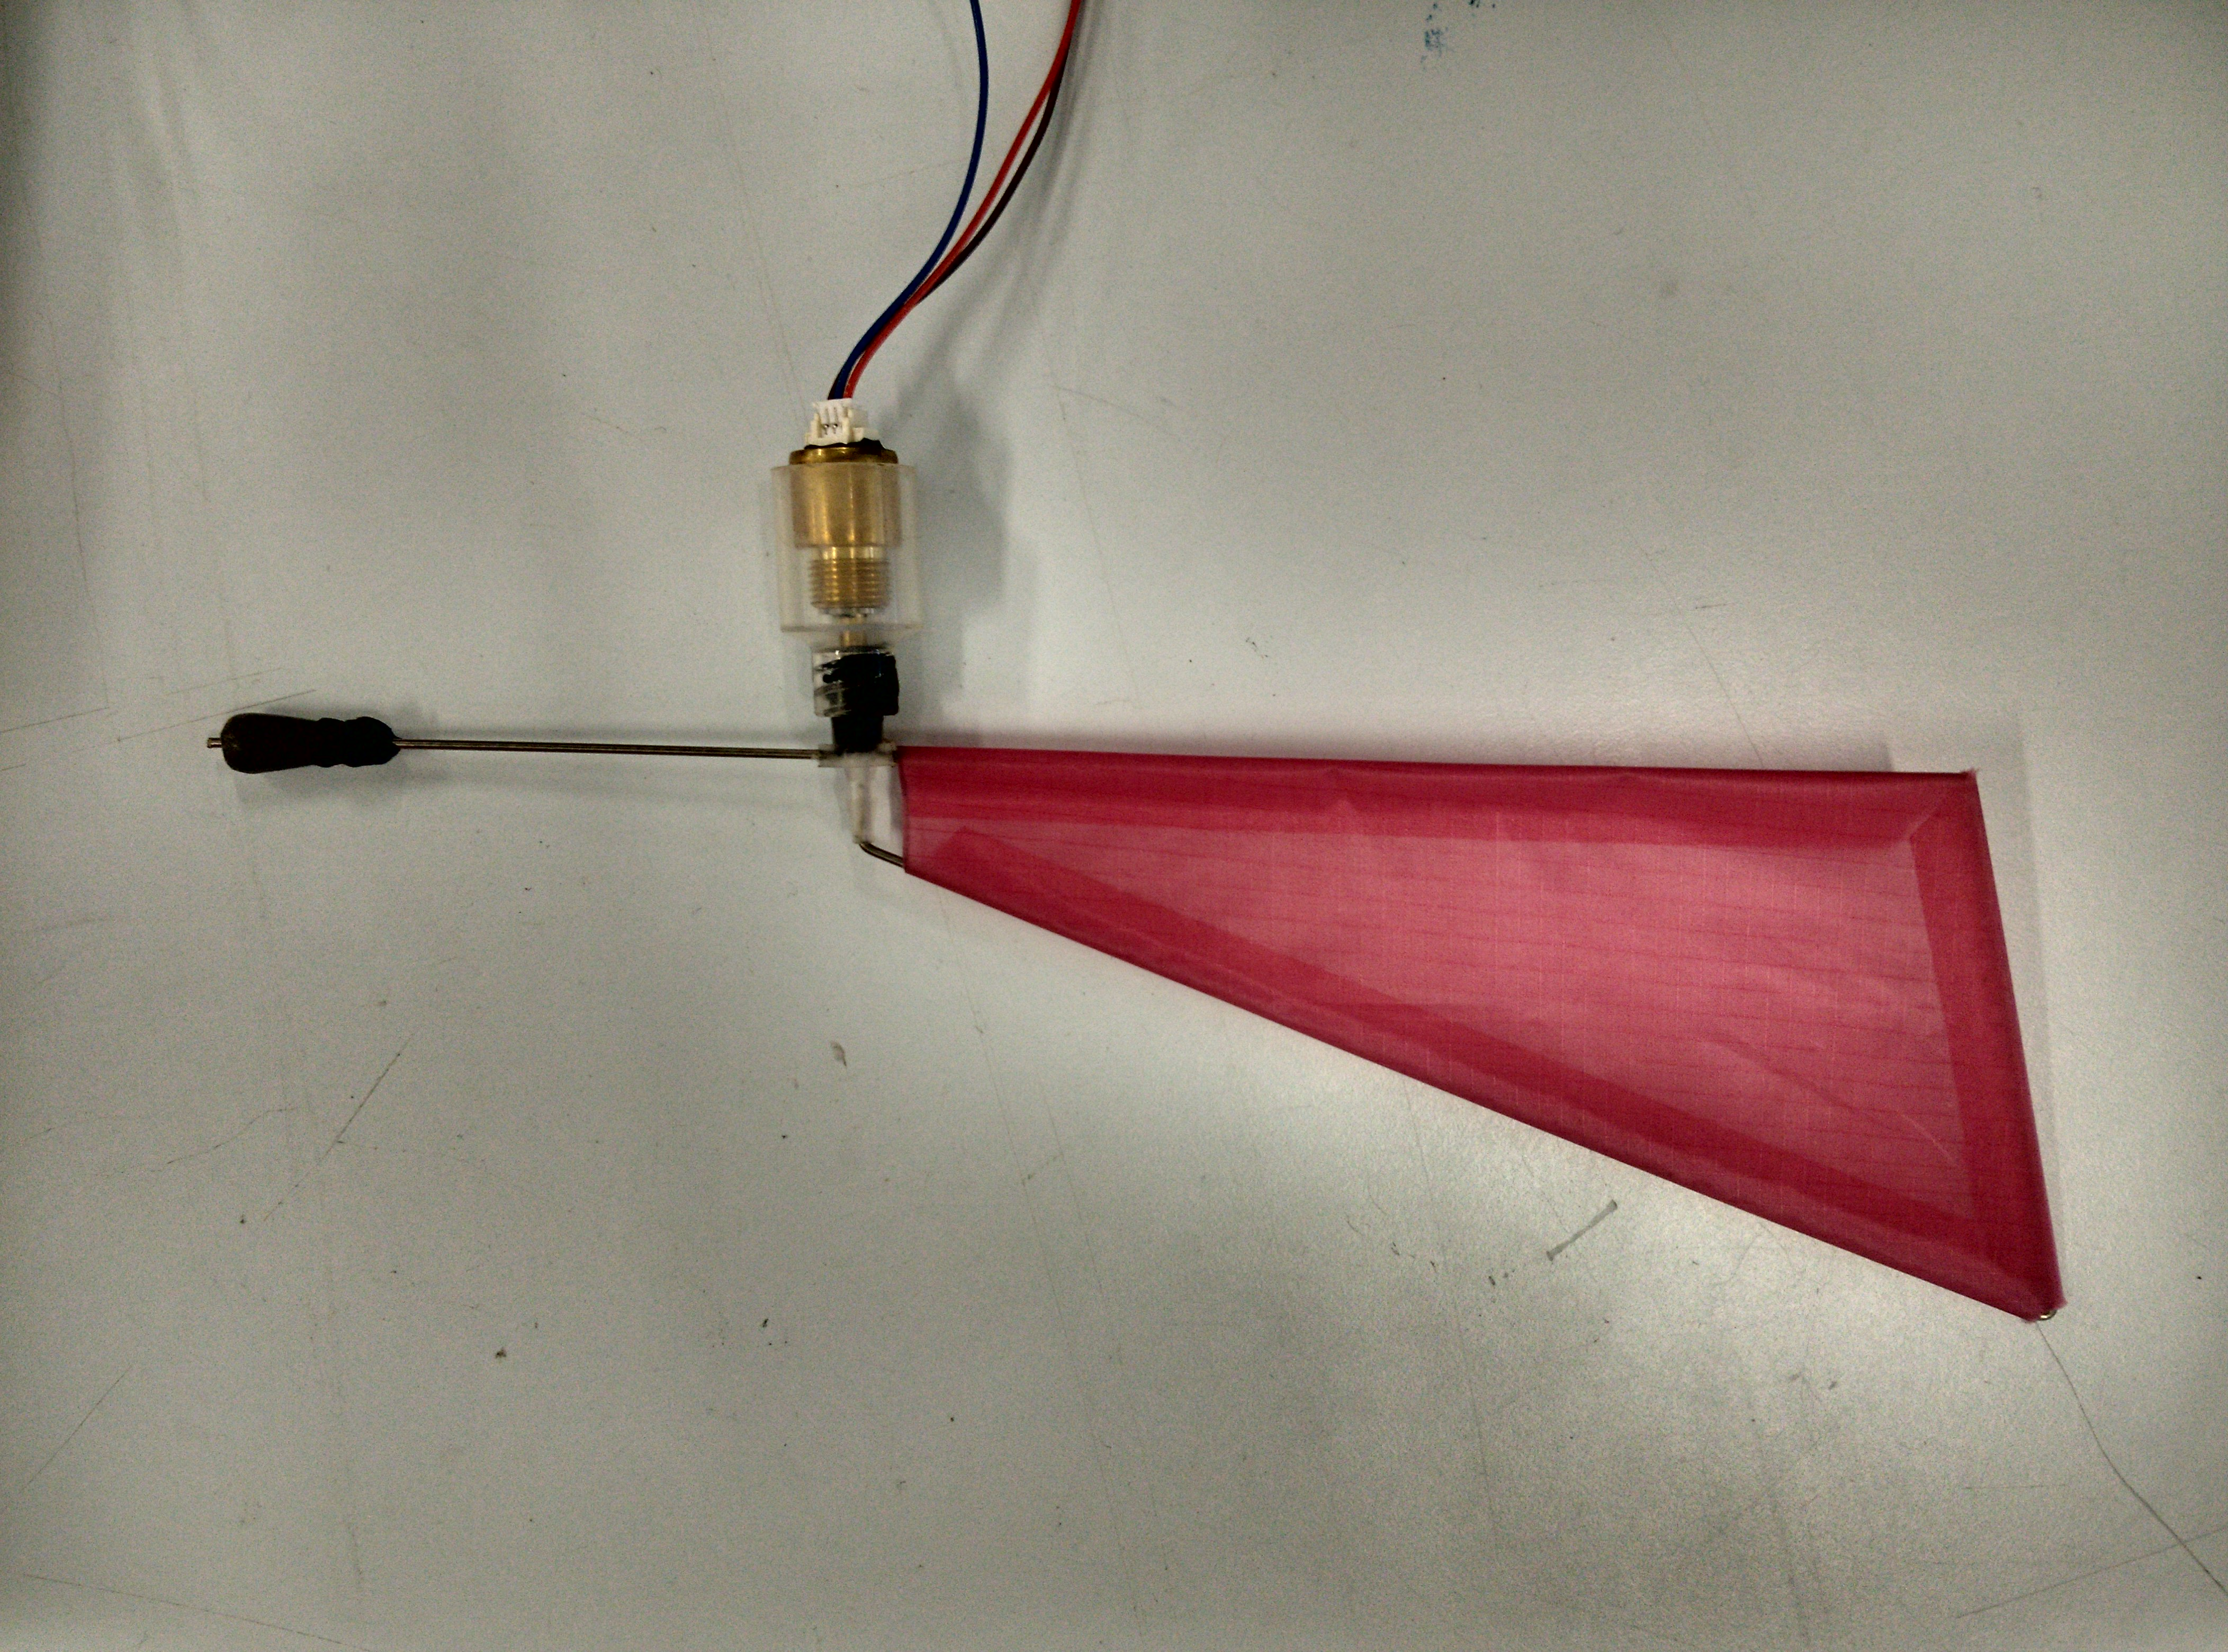
\includegraphics[scale=0.05,angle=0]{Images/WindCaptor.jpg}
    \caption{WindCaptor.}
    \label{fig:WindCaptor}
\end{figure}

\section{Servo-motor controller, pololu ship}

\begin{figure}[H]
\centering
    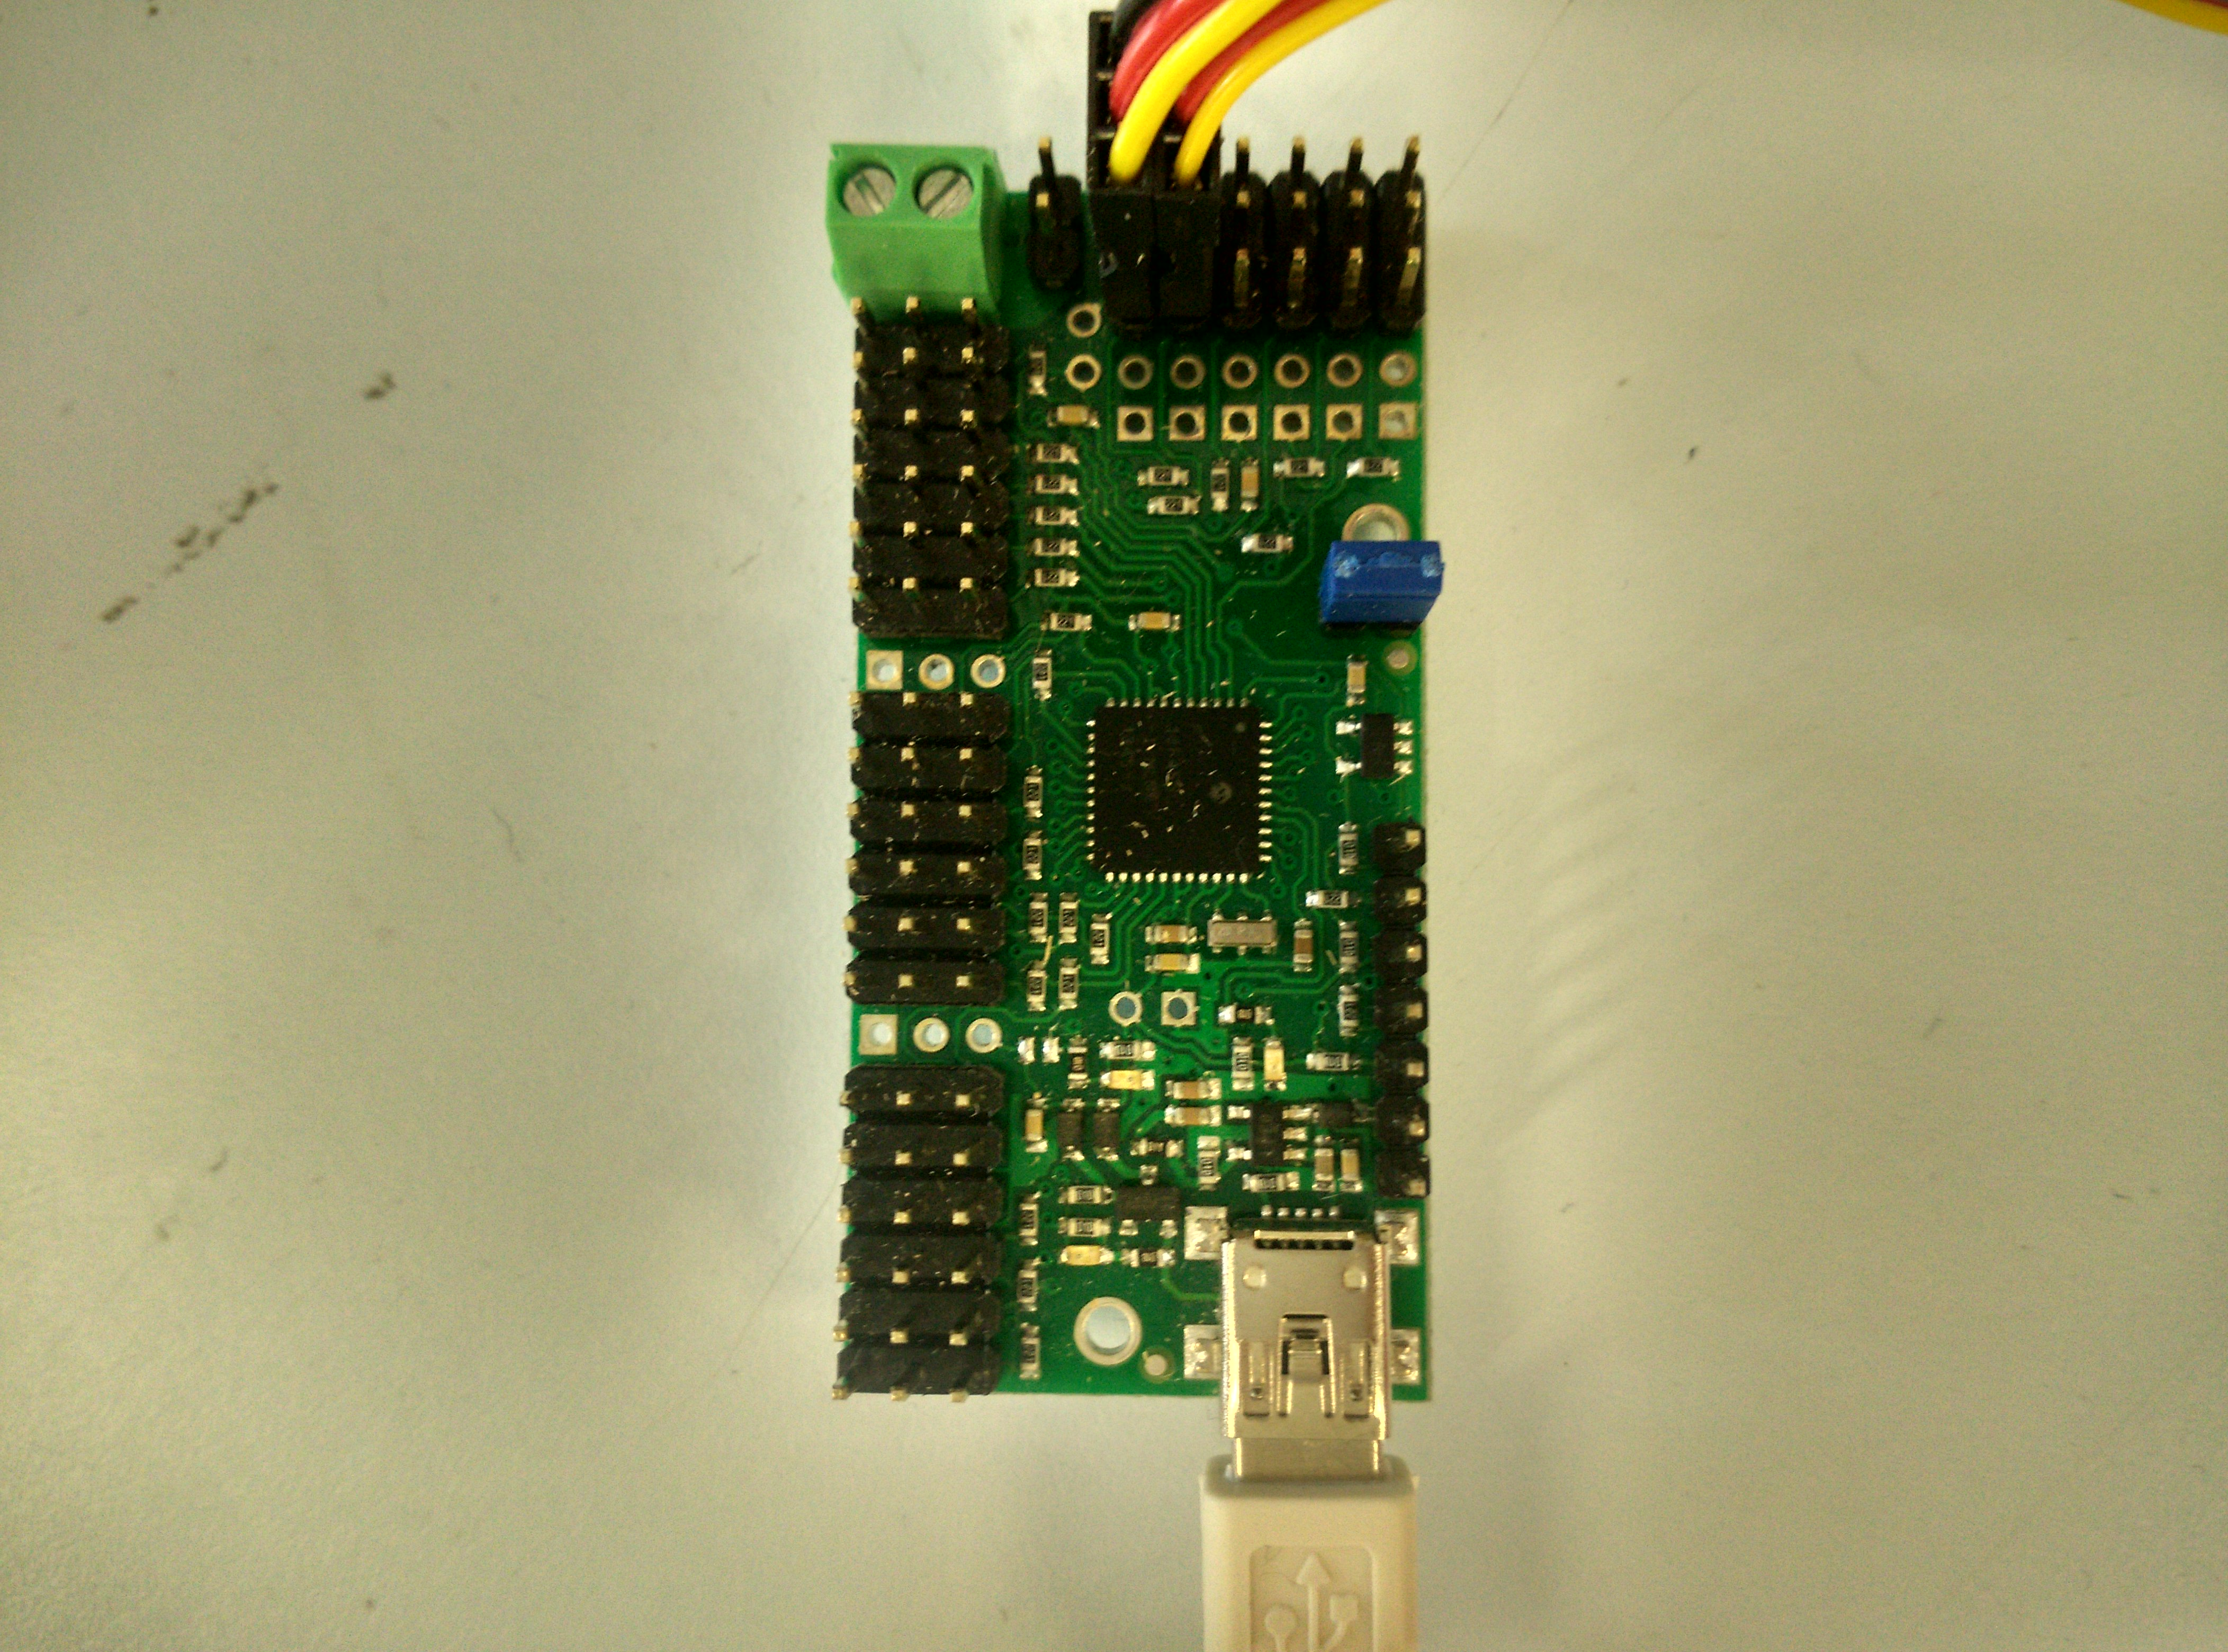
\includegraphics[scale=0.05,angle=0]{Images/Pololu.jpg}
    \caption{Pololu card.}
    \label{fig:Pololu}
\end{figure}

\section{GPS receiver}

\begin{figure}[H]
\centering
    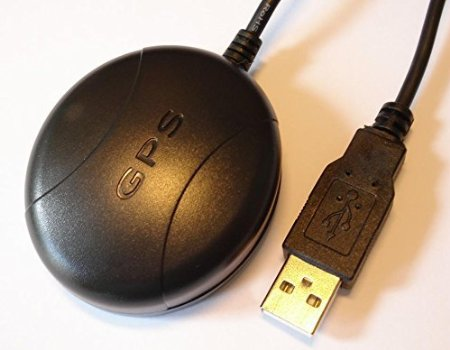
\includegraphics[scale=0.5,angle=0]{Images/GPS.jpg}
    \caption{Example of GPS receiver.}
    \label{fig:GPS}
\end{figure}

\chapter{Global architecture}

put photos here!!!



%----------------------------------------------------------------------------------------
%	PART III 
%----------------------------------------------------------------------------------------

\part{A voir}
\input{Part3}




\appendix
\part{Appendix}
\chapter*{Gaant diagram}

\begin{figure}[H]
\centering
    \includegraphics[scale=0.6,angle=0]{Images/GaantV1.PNG}
    \caption{Gaant diagram.}
    \label{fig:GaantV1}
\end{figure}

This Gaant diagram has been realized at the middle of the week and show what remains to be done in order to implement a solution to the project. I let at least 3 days to test the seam carving algorithm on the signals in order to find if the results are relevant. They are some other algorithms that can be used but they will be implemented if this one doesn't work.

The program which has been used in order to generate this diagram is \textbf{MindView 6.0}

%----------------------------------------------------------------------------------------
%	BIBLIOGRAPHIE
%----------------------------------------------------------------------------------------

%\addcontentsline{toc}{part}{Bibliography}
%\bibliographystyle{apalike-fr}
\nocite{*}
\bibliographystyle{plain}
\bibliography{bibliographie}


%----------------------------------------------------------------------------------------

\end{document}